 \documentclass[11pt, oneside]{article} 
\usepackage{geometry}
\geometry{letterpaper} 
\usepackage{graphicx}
	
\usepackage{amssymb}
\usepackage{amsmath}
\usepackage{parskip}
\usepackage{color}
\usepackage{hyperref}

\graphicspath{{/Users/telliott_admin/Dropbox/Tex/png/}}
% \begin{center} 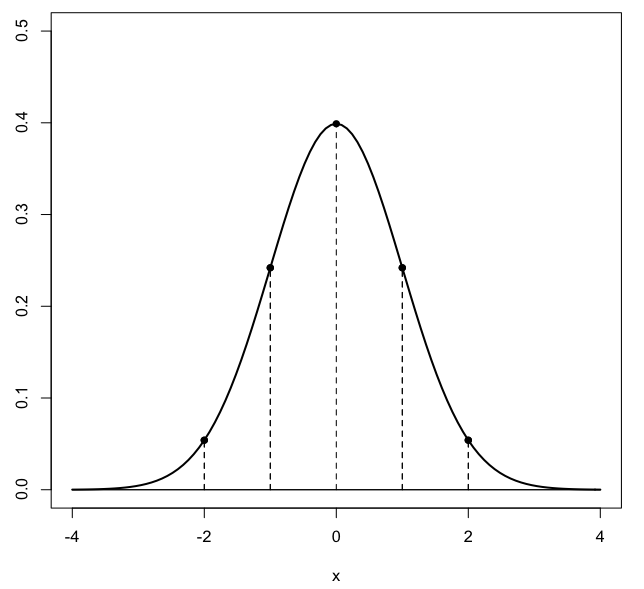
\includegraphics [scale=0.4] {gauss3.png} \end{center}

\title{Galois field $2^4$}
\date{}

\begin{document}
\maketitle
\Large

Let's take a quick look at GF($2^4$) before moving on to the main event (GF($2^8$)).

These are the polynomial equivalents of the binary numbers with 4 digits, all except $0000$.  There are 15 elements.

Degree 0:
\[ 1 \]
Degree 1:
\[ x \ \ \ \ x + 1 \]
Degree 2:
\[ x^2 \ \ \ \ x^2 + 1 \ \ \ \ x^2 + x \ \ \ \ x^2 + x + 1 \]

The new ones are degree 3.  Write them as binary equivalents:
\[ 1000 \ \ \ \ 1001 \ \ \ \ 1010 \ \ \ \ 1011 \]
\[ 1100 \ \ \ \ 1101 \ \ \ \ 1110 \ \ \ \ 1111 \]

\subsection*{irreducible polynomial}
We need an irreducible polynomial.  In GF($2^3$) we could choose from $x^3 + x + 1$ and $x^3 + x^3 + 1$.

Now we need a polynomial of degree 4.  Our method is to multiply together all polynomials of lesser degree and see what's missing.

A degree 4 is obtained either by multiplying a degree 3 times a degree 1, or by multiplying two of degree 2.  We'll see the details of this in the next chapter.

I did this and then, to see the patterns, wrote them all without the leading $1$ (and grouping by the next digit):
\begin{verbatim}
10 + 000 001 010 011 100 101 110 111
11 + 000 --- 010 011 100 --- 110 ---
\end{verbatim}

I find only 13, so 3 are missing.  These are

\begin{verbatim}
11001 11101 11111
\end{verbatim}

We choose $25 = 11001 = x^4 + x^3 + 1$ as the irreducible polynomial for GF($2^4$).

\subsection*{generator}
I first tried $\textbf{0x03}$ and found that it is not a generator for this field.  

Rather than guess again, I wrote a short script that calls the gmultiply routine.  It's modified to use the irreducible polynomial from above ($11001 =$ decimal $25$) and do the mod operation if $n > 15$.  

I'll put that code in a later chapter.  The output is

\begin{verbatim}
 2  4  8  9 11 15  7 14  5 10 13  3  6 12  1  2  4
 3  5 15  8  1  3  5 15  8  1  3  5 15  8  1  3  5
 4  9 15 14 10  3 12  2  8 11  7  5 13  6  1  4  9
 5  8  3 15  1  5  8  3 15  1  5  8  3 15  1  5  8
 ..
 15  3  8  5  1 15  3  8  5  1 15  3  8  5  1 15  3
\end{verbatim}

Unexpectedly, 2 and 4 are generators but 3 and 5 are not.  Although one can look for repeated values like $5$ in the row starting with $3$, an easier way is to scan for $1$ in the middle of the table.

So
\begin{verbatim}
 0010
 0010
 ----
 0100 => 0100
 0010
 ----
 1000 => 1000
 0010
 ----
10000
11001 mod
-----
 1001 => 1001
 0010
 ----
10010
11001 mod
-----
 1011 => 1011
..
\end{verbatim}
I won't show the whole thing.

I obtained
\begin{verbatim} 
0100 1000 1001 1011 1111 0111 1110 0101
1010 1101 0011 0110 1100 0001 0010
\end{verbatim}
and compare that with what the Python code produced:
\begin{verbatim}
 2  4  8  9 11 15  7 14  5 10 13  3  6 12  1  2
\end{verbatim}

That's a match.  With the powers, we can compute a table of logarithms.  

Here they are:  the elements are in the first row and the logarithms below.
\begin{verbatim}
 2  4  8  9 11 15  7 14  5 10 13  3  6 12  1  2
 1  2  3  4  5  6  7  8  9 10 11 12 13 14 15 16
\end{verbatim}

According to this, 7 and 14 should be multiplicative inverses because their logarithms add to 15, whose anti-logarithm is 1.

Try it:

\begin{verbatim}
    0111 =  7
    1110 = 14
    ----
    111
   111
  111
  ----
 101010
 11001 mod
 -----
  11000
  11001 mod
  -----
      1
\end{verbatim}

This is pretty tedious.  I wrote some code to carry out the procedure, and check the above multiplicative inverses.  They are all correct.

The last thing is to try an example of the extended Euclidean algorithm.  Find the multiplicative inverse of 5.
 
\begin{verbatim}
    a     b     q      bq     r
11001   101   110   11110   111
  101   111     1     111    10
  111    10    11     110     1
-----
111 = 11001 - (110)101
 10 = 101 - (1)111
  1 = 111 - (11)10
    = 111 - (11)[101 - (1)111]
    = (10)111 - (11)101
    = (10)[11001 - (110)0101] - (11)101
    = (1100)101 + (11)101
    = (1111)101
    = (15)(5)
\end{verbatim}
which is correct.  The log of $5$ is $9$ and the log of $15$ is $6$ and the sum of the logs is $15$, which is the anti-log of $1$.

\end{document}